\chapter{Background}\label{ch:Background}

In recent years, deep learning has become somewhat of a buzzword within the world of computing, but not without good reason. Deep learning models, those comprised of a large number of processing layers in order to learn multiple abstracted representations of the data provided, have consistently been shown to outperform other machine learning techniques, especially in the field of computer vision \cite{lecun_deep_2015}. As the field of deep learning increases in scope every day, this Chapter will focus primarily on the world of deep learning in a computer vision context. A brief introduction to deep learning will be provided, before looking at how these methodologies have been applied to computer vision, specifically Convolutional Neural Networks (CNNs) and their use in object detection. Literature focusing on computer vision in a marine cetacean space will be explored, as well as the current space of fine-grained computer vision. An introduction to photo-identification is also provided. 

\section{A Brief Introduction to Photo-Identification}\label{ch:Background,sec:photo-id}

Photo-identification, often abbreviated to photo-id, is one of the main mark-recapture methods utilised by cetacean researchers for tracking and identifying individuals in a survey area in a non-invasive manner (compared to methods such as tagging). This methodology involves the undertaking of a large scale monitoring of a survey area, usually occurring at sea through the use of a small boat, although monitoring from coastlines or aircraft may also be utilised \cite{payne_long_1986, forney_seasonal_1998, wursig_methods_1990}. More recently, the use of citizen science has also began to be incorporated within photo-id surveys where evidence exists of smaller species population densities over large areas which may make full-scale monitoring infeasible \cite{gibson_using_2020, cheney_integrating_2013}.

Initially utilised for the tracking of individual distinctive animals within a species \cite{caldwell_evidence_1955, schevill_daily_1960}, the methodology was quickly adapted to large-scale monitoring of whole pods. The methodology is primarily utilised during cetacean health monitoring and abundance estimation studies, with proven use cases on a variety of cetacean species such as Indian Ocean humpback dolphins (\textit{Sousa plumbea}) \cite{sharpe_indian_2019}, Risso's dolphins (\textit{Grampus griseus}) \cite{miragliuolo_rissos_2004}, and killer whales (\textit{Orcinus orca}) \cite{bigg_assessment_1982}. Outside of cetaceans, photo-id has further found use studying other marine life such as whale sharks (\textit{Rhincodon typus}) \cite{holmberg_estimating_2009}, sea turtles (both \textit{Chelonia mydas} and \textit{Eretmochelys imbricata}) \cite{reisser_photographic_2008}, and Florida manatees (\textit{Trichechus manatus latirostris})  \cite{langtimm_survival_2004}. 

As can be seen from the examples of species where photo-id is utilised, this methodology for mark-recapture relies on the species having some form of individually identifiable markings, similar to human fingerprints. Typically, this identifying information is located on a part of the body which is likely to breach the water at some point during an encounter, although examples of underwater photo-id do exist in literature though are not yet commonplace \cite{vanbressem_visual_2018}. Depending on the species of animal, different parts of the body are the primary identifying location; for dolphins this is usually the dorsal fin whilst for whales this is primarily the fluke, or callosities if present \cite{vernazzani_eastern_2013, arnbom_individual_1987, constantine_abundance_2012, sharpe_indian_2019, baird_population_2009}. See Figure \ref{fig:body-parts} for examples.

\begin{figure}
	\begin{center}
		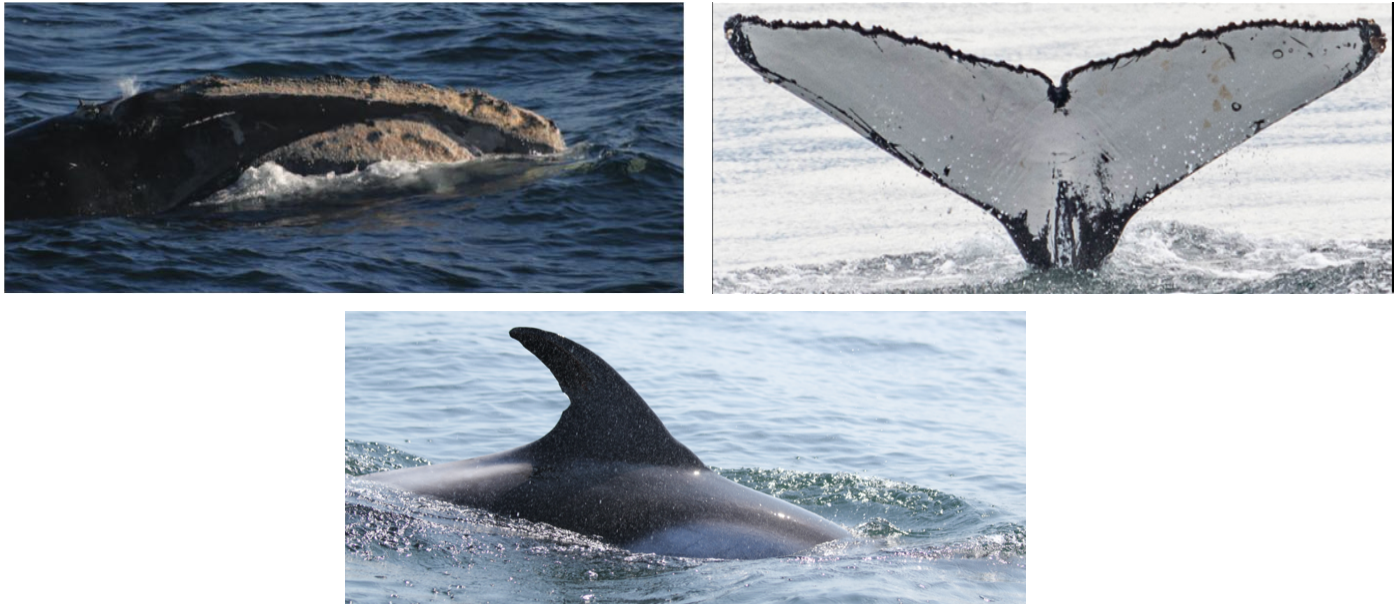
\includegraphics[scale=0.6]{Chapter2/figs/body-part-examples.png}
	\end{center}
	\caption{Examples of the main body parts utilised in cetacean photo-id. Left: callosities present on the head of a northern right whale (\textit{Eubalaena glacialis}) \cite{perrin_encyclopedia_2009}. Right: fluke of a humpback whale (\textit{Megaptera novaeangliae}) \cite{cheeseman_happywhale_2019}. Bottom: dorsal fin of a common bottlenose dolphin (\textit{Tursiops truncatus}) \cite{trotter_ndd20_2020}.
	}
	\label{fig:body-parts}
\end{figure}

During photo-identification surveys, researchers will often focus on long lasting markers such as body-part shape, nicks, notches, and pigmentation which have been shown to be stable throughout the life of the animal \cite{wursig_photographic_1977, lockyer_observations_1990, mann_cetacean_2000}. In some cases secondary markers, those which may heal and are thus not stable such as scarring, may also be utilised for identification. These secondary markers may be anthropogenic, for example from collision with a vessel, or natural, for example from encounters with prey. Scarring is of particular use when identifying Risso's dolphins who are well known for the persistent nature of their scarring, which is thought to occur due to a loss of pigmentation when their scars heal \cite{mariani_analysis_2016}. Pigmentation also occurs in other cetacean species such as striped dolphins (\textit{Stenella coeruleoalba}) and has been used for photo-identification where it can be considered a primary marker \cite{rosso_colour_2008}.

Regardless of the species being analysed or the body-parts used during the photo-id process, some assumptions must be universally made. For one, all of the markers must be considered stable, that is, they must not fade over the years. Even if a photo-id study only occurs over a few years, the markers utilised must be stable enough so that if another survey is conducted in the same area in later years, individuals from the first study must still be identifiable, providing useful information to health assessments, population estimates, and residency surveys. This stability reduces false negatives, where one individual is recorded as multiple over time. Second, the markers must be considered individually unique. Those chosen to identify an individual must not overlap with other individuals in the survey area. This reduces the chance of false positives, where multiple individuals are recorded as one. Chosen markers must also allow for a consistent re-sighting probability over time. This is critical for abundance estimates,  ensuring that an individual's chosen markers providing it with the same chance of being spotted one year as another. As such, it is extremely important that photo-id methodologies are standardised, both at an international level and between researchers in the same organisations. This process began in 1988 through workshops held by the International Whaling Commission, with further recommendations published in 2015 by Urian \textit{et al.} \cite{hammond_individual_1990, urian_recommendations_2015}.

Because of the assumptions which must be adhered too, as well as the manual nature of the photo-id process, there are many downsides. Being able to identify individuals relies on high quality photographs. Thanks to the advent of digital photography and the relative inexpensiveness of cameras capable of capturing large megapixel images, this is less of an issue than before, although it still must be considered. Surveys can also only be undertaken in good weather conditions in terms of sea state and lighting, both of which can affect the chance of an accurate match. These conditions are harder to meet in some areas of the world, reducing the suitability of photo-id for some geographic areas. Conditions, as well as the nature of the animal itself, may make photographing both sides of the individual impossible. Markings are rarely duplicated on both sides of an individual, and thus not having both sides may make matching difficult. For example, an individual may have an extremely distinctive marking on the left side of their dorsal fin however if only the right side of the individual has been captured, when the left side is also eventually photographed it may be labelled as a new individual as no previous examples of the individual's left side exist in the catalogue. 

Furthermore, photo-id as a whole is extremely labour intensive. Unlike land based camera trap systems, marine based photo-id surveys require a large human effort. Staff are needed not just for photographic purposes, but also for piloting of vehicles. As the surveyed animals are free roaming, large spatial areas must be covered, and there is no guarantee of encountering them during a given day. Back on land, the captured photographs must then be manually worked through and the individuals in them identified. This can often take longer than the entire data collection period. Thanks to the labour intensiveness  of the photo-id process, it can also be extremely costly to undertake. Staff need to be paid, vehicles need to be fuelled, and equipment must be maintained. Because of this, any solutions which may speed up the photo-id process would be welcomed both by researchers and their funding bodies. 

\section{A Brief Introduction to Deep Learning}\label{ch:Background,sec:DLIntro}

Deep learning, a subfield of machine learning, aims to create artificial networks to complete tasks, i.e. learn, in a similar way to how neurons in the human brain operate. These computational models are often multiple neurons deep, known as layers, with lower layers representing basic abstractions, building up from this as you go \textit{deeper} into the network, resulting in final layers of neurons which, based on information passed to them from lower levels, can begin to provide estimations of answers to a given problem. It is in this way that deep learning methods differ from older machine learning techniques, which were far more constrained in how data could be represented. Considerable domain expertise was required to design a feature extractor allowing for raw data values, such as pixels, to be transformed into a feature vector suitable for a model to be able to detect or classify the input. 

Deep learning models in contrast are capable of performing classification on raw data values through multiple layers of simple non-linear transformations. For example in the case of computer vision, lower layers of neurons may be optimised to learn lines and basic shapes, middle layers may be optimised to learn more complex ideas such as how these lines and shapes fit together, with the final layers providing an output of object label (e.g. \texttt{dolphin}). It should be stressed however that the features these layers are looking for are not specified by humans, but rather learned from the data by updating their weights and biases, predominantly through stochastic gradient descent and backpropagation  \cite{hecht-nielsen_iii.3_1992}. This is very similar to how the brain learns from the multi-modal data it receives from the body, capturing the intricacies of massive amounts of data using a connection of smaller optimised neurons. 

This ambition to create networks similar to how the brain operates stems mainly from work undertaken in 1943 by McCulloch and Pitts \cite{mcculloch_logical_1943} in an attempt to understand how neurons in the brain allow for the understanding of complex patters. This model formed the basis of future work into machine learning, and thus deep learning. This work continued at small scale for many years. It has only been recently thanks to advances in availability and power of the computing resources available has deep learning research accelerated. The transition away from model training on CPUs to multiple high-powered GPUs has been one of the largest advancements in deep learning, allowing for a significant speed-up in the train time for these models, resulting in much more prototyping in a smaller time frame. Further to this, the advent of cloud computing has allowed for much more cost-effective model development. Thanks to the Pay As You Go model of computing now commonplace, cloud providers such as Microsoft, Amazon, and Google have eliminated the need for researchers to procure their own hardware required for training, which can in some cases be prohibitively expensive. 

More so, advances in deep learning have been helped greatly through the development of standard development frameworks. Google's Tensorflow \cite{abadi_tensorflow:_2016} and Facebook's PyTorch \cite{paszke_automatic_2017} allow for researchers to develop models much faster than previously due to their reduction in the amount of boiler-plate code needed, with these frameworks often doing a lot of the \textit{heavy lifting} in the background. Further advances have been made through the availability of high quality coarse-grained datasets such as MNIST \cite{lecun_gradient-based_1998}, Caltech-256 \cite{griffin_caltech-256_2007}, and ImageNet \cite{deng_imagenet:_2009} allowing for common baselines to be adopted by the computer vision community and for the introduction of transfer learning, allowing for the reuse of models trained in one task to be utilised for another \cite{pan_survey_2010}. Furthermore, additional regularisation techniques have provided improvements to model accuracy. Notable examples of this in literature which are now commonplace in deep learning models include dropout \cite{srivastava_dropout:_2014}, batch normalisation \cite{ioffe_batch_2015}, stochastic gradient descent with warm restarts \cite{loshchilov_sgdr:_2016}, mixup \cite{zhang_mixup:_2017}, as well as various forms of data augmentation. 

\subsection{Supervised and Unsupervised Learning}\label{ch:Background,sec:DLIntro,sub:supervisedVsUnsupervisedLearning}
Within machine learning as a whole, all tasks can be placed into two categories, supervised or unsupervised learning. 

\textbf{Supervised learning} tasks are those where prior knowledge of what the output value should be, also known as a ground truth, is known. This learning is thus often performed for classification, mapping inputs to a defined set of outputs, or in regression where an input is mapped to a continuous output function. As such, supervised learning's goal can be seen as attempting to understand and generalise the relationship between a set of inputs and a set of outputs. 

This generalisation is performed by splitting the available data into training and test sets, with the former being used to train the model and the latter being used to test the model's performance on previously unseen data. Both the training and test set contains ground truth data, but only the training set's influences the generalisation of the model. For example, in the case of a dog or cat classifier a dataset may contain 1000 images, some labelled as \texttt{dog} and some as \texttt{cat} (the ground truths). This data will then be split randomly into a training and test set; common splits often allocate 80-90\% of the data for training with the remaining set used for testing. The classifier will then iterate through the training set, using the ground truth values along with algorithms such as stochastic gradient descent (discussed in more detail in Section \ref{ch:Background,sec:DLIntro,sub:stochasticgradientdescent}) to train each neuron's weights and biases in a way to best generalise the model. After training has been completed the model will then be evaluated against the test set, with each of the unseen images being classified. These predicted classifications will then be compared to the unseen ground truths in order to provide an evaluation metric of the model's performance. 

\textbf{Unsupervised learning} tasks are, in contrast, those where prior ground truths for your data are not available. As such, no classification can be performed using this method, however it is often used for clustering and aiding in understanding of the underlying data structure. These unsupervised algorithms, such as K-Means clustering \cite{hartigan_algorithm_1979}, are not given any guidance on how to define the data into clusters but are rather left to discover interesting structure on their own. 

Taking our dog and cat data again as an example, it is clear how this data could be clustered in an unsupervised manner. Asking the clustering algorithm to provide two clusters for the data  (e.g. $K = 2$) , a model could be trained to split the data with all dogs in one cluster and all cats in the other, without having to be told which images are dogs and which are cats. 

\subsection{The Stochastic Gradient Descent Algorithm}\label{ch:Background,sec:DLIntro,sub:stochasticgradientdescent}
In order to generalise our deep learning models, we need to be able to optimise the weights and biases within each individual neuron. Most commonly, this is performed using gradient descent to minimise a loss function (a measure of distance between ground truth and prediction)  in such a way that weights are updated in the \textit{opposite} direction of the gradient of the loss function. As such, we follow the direction of the slope of the surface created by the loss function downhill iteratively until we reach a minima, an area where the loss is lowest \cite{ruder_overview_2016}. Before the advent of deep learning and big data, it was common for the whole dataset to be used to compute the gradient at each iteration; however due to the size of modern day datasets this is no longer possible due to the computational cost this would impose on the system. As such, batches of the dataset are often used to give an estimation of the overall loss gradient.

In order to reach this minimum, a process known as stochastic gradient descent (SGD) is most commonly used. At each iteration of SGD, a batch will only contain one randomly selected training example. The loss for this example is calculated, and used to step down the gradient slope, rather than the sum of the loss' gradient over all training examples. As we only take one example per iteration, the path taken down the slope to the minima is far noisier and random than the path obtained from using all examples, hence the \textit{stochastic} nature of the gradient descent. This stochastic nature does result in a longer convergence time to the minima compared to a regular gradient descent, however this is outweighed by the reduction in computational expense. The use of SGD often leads to a good set of model weights quickly compared to other, more elaborate techniques \cite{bottou_tradeoffs_2008}. 

In recent years there have been efforts to modify SGD in an attempt to improve model optimisation. The most commonly seen optimisations within production code include SGD with warm restarts \cite{loshchilov_sgdr:_2016}, Momentum \cite{qian_momentum_1999}, RMSProp \cite{tieleman_lecture_2012}, Adam \cite{kingma_adam:_2014}, and AMSGrad \cite{reddi_convergence_2019}. All of these optimisations attempt to stop the problem of getting stuck in local minima rather than the global minimum of the overall loss function. However, recent studies show that the problem of local minima is not as big as first thought and, regardless of initial conditions, vanilla SGD rarely gets stuck in local minima \cite{dauphin_identifying_2014, choromanska_loss_2015}.

\subsection{Backpropagation}\label{ch:Background,sec:DLIntro,sub:backprop}
As discussed in Section \ref{ch:Background,sec:DLIntro,sub:stochasticgradientdescent}, we have seen how weights and biases in each neuron can be learnt and optimised using SGD. However, it is important that we also discuss how the gradient is computed. This computation can be performed relatively quickly using backpropagation, or the backward propagation of errors algorithm. Before delving \textit{too deep} into deep learning, it is of imperative importance to understand backpropagation; it is after all often cited as one of the cornerstones of deep learning \cite{alber_backprop_2018}.

Backpropagation was originally described in Linnainmaa's masters thesis \cite{linnainmaa_representation_1970}, although it's effect was not fully realised until 1986, when Rumelhart \textit{et al.} discussed the advantages to using backpropagation over other learning approaches \cite{rumelhart_learning_1986}. Whilst multiple attempts have been made to improve the original algorithm \cite{bengio_use_1994, lillicrap_random_2014, lee_difference_2015, nokland_direct_2016, liao_how_2016}, these are rarely adopted by deep learning researchers as little improvement can be gained from them compared to the overhead of modifying existing deep learning frameworks to incorporate the changes. 

The standard backpropagation algorithm to compute the gradient of the loss function w.r.t a model's layers is, in essence, the chain rule (a formula for computing the derivative of multiple functions). Working backwards through the network, the last layer's gradient is first calculated providing a partial calculation of the overall network's gradient. This is then used to efficiently calculate the layer above's gradient, propagating information regarding the loss and how weights should be changed throughout the network. This backwards propagation is a far more computationally efficient way of calculating the overall loss gradient compared to calculating each layer's gradient loss in isolation. Further efficiencies have been made thanks to deep learning frameworks implementing backpropagation in a way that takes advantage of GPUs, leading to extremely efficient computations when performing deep learning tasks such as object detection and other computer vision tasks.


\section{Deep Learning for Computer Vision}\label{ch:Background,sec:DLforCV}

The field of computer vision, allowing computers to gain and interpret knowledge from image and video data, is one area where deep learning has excelled. Generalisable concepts such as CNNs have quickly become commonplace for solving computer vision tasks, in most cases replacing the need for hand-crafted pipelines specialised to the task at hand, thanks to their ability to learn complex patterns in data where there is a strong spatial and temporal dependency between the values. This ability is essential for processing image data which is, at it's most basic level, a matrix of pixel values. These matrices are three dimensional, representing an image's height, width, and depth, where depth is dependant on the colour model used to represent the image. The most common of these models is RGB which has channels representing the red, green, and blue visual light present in an image; as such a matrix representing an RGB image will have a depth of three. Other colour models have varying depth values, a greyscale image would have a depth of one for example, whilst a CMYK image would have a depth of four. As can be imagined, these matrices can very quickly reach massive sizes. An RGB image at 1080p resolution for example would require a matrix of size 1920x1080x3, or 6,220,800 values. CNNs allow us to reduce the image down to a more workable form whilst still retaining key features which will allow us to infer predictions.

\subsection{Convolutional Neural Networks}\label{ch:Background,sec:CNN,sub:CNN}
Modern CNNs are composed of three main layer types; convolutional layers, pooling layers, and fully connected layers. Each of these layers will perform some operation on the input matrix passed to it, and provide a transformed output to the subsequent layer(s). These layers can be stacked in various orientations to build different CNN architectures.

\subsubsection{Convolutional Layers}\label{ch:Background,sec:CNN,sub:CNN,subsub:convolution}

The convolutional layer is the workhorse of the CNN, performing the vast majority of the operations required. Convolutional layers utilise what is known as a kernel in order to efficiently extract features from an input image matrix. A kernel is a matrix, most commonly 3x3 or 5x5 in size, which represents some weighting refined through training. This kernel is slid over the input data computing the dot product between the weights and the section of the input matrix it is currently over, before summing these into a single value. This gives an output matrix of features represented by the weighted sum of the input, known as a feature map. These feature maps generally represent basic shapes at shallow levels, which are the  built on as the model gets deeper, representing more complex shapes as you progress. 

The kernel process can be performed multiple times over the same input using different weightings, giving multiple output feature maps. In the case where there are multiple input dimensions (such as an RGB image), kernels are required to operate over all dimensions. As such, the resulting feature maps are summed element-wise, along with some bias term, to produce a single output map. 

The size of the kernel as such determines the number of input features which are combined to give the new output feature map, although the size of the resulting map is determined also by two other properties; stride and padding. Stride refers to the distance in pixels the kernel will move when performing the next input mapping. For example, a stride of 1 would result in the kernel sliding along one pixel value each time, resulting in an output feature map of equal size to the input, whereas a stride of 2 would skip every other pixel, reducing the output feature map by half. 

A problem can arise during convolution when the kernel reaches the edges of the input matrix. As there is nothing past the edge values, these values must be trimmed as they are never in the centre of the kernel. This can cause the reduction of the matrix, as some values are never utilised, which may be detrimental when we require an output feature map which is the same size as that of the input. As such, padding can be performed. This technique places zeros around the edges of the input matrix, expanding it's size and allowing pixel values formerly at the edges to be utilised by the kernel. A visual representation of how convolution is performed can be seen in Figure \ref{fig:kernels}.

\begin{figure}
	\begin{center}
		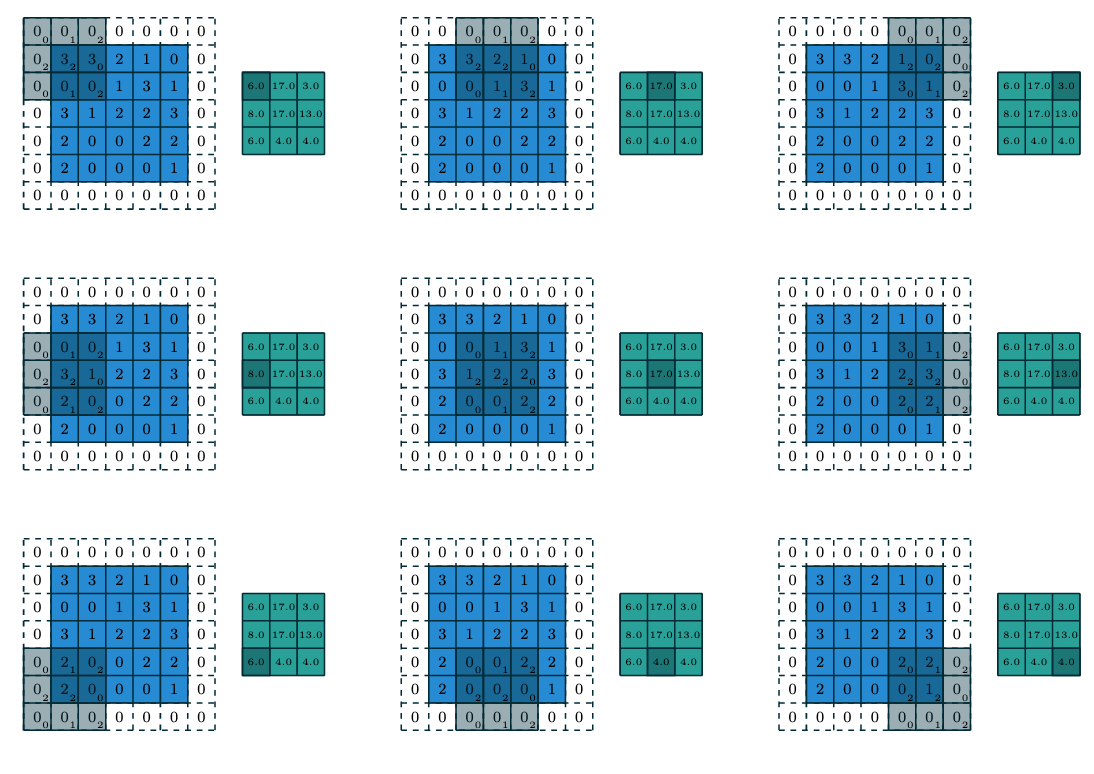
\includegraphics[scale=0.45]{Chapter2/figs/kernel.png}
	\end{center}
	\caption{A visual representation of convolution. A kernel, represented by the grey squares, operates over a padded input matrix, blue, with a stride of 2 to produce an output feature map, green. Note that the kernel's weights are denoted by the number in the lower right of each box and the input pixel value is denoted by the number in the middle of each box. \cite{dumoulin_160307285_2018}}
	\label{fig:kernels}
\end{figure}


\subsubsection{Pooling Layers}\label{ch:Background,sec:CNN,sub:CNN,subsubsec:pooling}

Pooling layers help reduce the computational complexity of the convolutions performed by the CNN. This is achieved by reducing the spatial dimensions of the input ready for the next convolutional layer through the use of some function. Pooling only affects the width and height of the input, not the depth, as all depth channels are required to keep the colour mapping of the image intact. 

Pooling as such inevitably leads to a reduction in the amount of information available to subsequent layers; this is advantageous however as it leads to less computational complexity, aiding in the minimisation of overfitting in the model. 

A number of different pooling layer architectures exist in literature, such as max pooling, average pooling \cite{boureau_theoretical_2010}, and stochastic pooling \cite{zeiler_stochastic_2013}, although more recent architectures favour the use of strided convolutions, rather than pooling, to reduce the size of the output feature map.

\subsubsection{Fully Connected Layers}\label{ch:Background,sec:CNN,sub:CNN,subsubsec:fullyConnected}

Fully connected layers take feature maps produced by the preceding convolutional and pooling layers and reduce these down to a single $N$-dimensional vector, where $N$ represents the total number of classes and each dimension's value is the probability of the class. These probabilities are achieved using a softmax activation function, which takes the exponents of each input and normalises them by the sum of all inputs, giving values between 0 and 1. Outputted $N$-dimensional vectors can then be considered a feature map in their own right for further processing \cite{krizhevsky_imagenet_2012} or as a category for classification as the last layer of the network \cite{girshick_rich_2014}.

\subsubsection{Layer Architectures}\label{ch:Background,sec:CNN,sub:CNN,subsub:layerArchitecture}

Using the three layer types described above it is possible to create, in theory, an infinite number of CNN architectures all with different amounts and combinations of layers. There is no guarantee that every possible architecture will perform well however (indeed, one possible combination would be a single fully connected layer, which would not perform well at all). Whilst it may be advantageous for certain areas of research to create their own custom CNN architecture, either through trial and error or the more recent approach of Neural Architecture Search \cite{elsken_neural_2018}, this is not applicable for most cases. For the vast majority of cases, there exists in literature well-defined generalised CNN architectures, and it is often these architectures which are utilised for computer vision tasks. 

LeNet \cite{lecun_gradient-based_1998} was the first well defined CNN architecture. LeNet was only 7 layers deep, but performed well enough to be applied by some banks for automatic recognition of numbers on cheques. It wasn't until around 2012 that more attention was paid to these defined architectures however, thanks to AlexNet \cite{krizhevsky_imagenet_2012}. Utilising a similar but deeper architecture to LeNet, with more filters and a larger number of stacked convolutional layers, AlexNet also included now common CNN building blocks such as dropout \cite{srivastava_dropout:_2014}, max pooling \cite{boureau_theoretical_2010}, and ReLU activation functions; the most popular non-linear activation function currently in deep learning, especially in computer vision \cite{he_delving_2015}. 

The activation function is responsible for deciding which neuron in the layer passes it's value to the layer below by computing the weighted sum of the inputs and passing the result through a non-linear function. ReLU's non-linear function returns 0 for any negative value, or for any positive value $x$, it returns $x$. This can be written as $f(x) = max(0,x)$, and visualised in Figure \ref{fig:relu}. It is this non-linearity that allows for backpropagation to occur.

\begin{figure}
	\begin{center}
		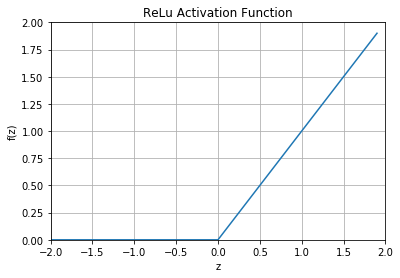
\includegraphics[scale=0.6]{Chapter2/figs/relu.png}
	\end{center}
	\caption{A visualisation of the ReLU Activation Function}
	\label{fig:relu}
\end{figure}

 In 2014, Google introduced GoogleNet, also known as an Inception architecture, to the ILSVRC14 competition \cite{szegedy_going_2015}. This net achieved a top-5 error rate of 6.67\%, very close to what untrained humans could achieve on the competition dataset. This was achieved through a 22 layer deep CNN utilising several small convolutions, reducing the number of parameters from 60million in AlexNet to 4million in GoogleNet. 

Finally ResNet was introduced a year later at ILSVRC15. This architecture can be as large as 152 layers deep, and achieved a human-beating top-5 error rate of 3.57\% \cite{he_deep_2015}. Shallower versions of ResNet exist, such as ResNet50 and ResNet101, which are 50 and 101 layers deep respectively. 

\subsection{Object Detection}\label{ch:Background,sec:objectDetection}
As discussed, CNNs are now one of the main tools available for computer vision tasks. Object detection tasks are no exception, with CNNs now being utilised en masse. These tasks concern themselves with attempting to identify and segment distinct classes of objects found in images and video, and is often performed in one of two ways. 

\subsubsection{Region Proposal Networks}\label{ch:Background,sec:objectDetection,sub:RPN}
The first, known as a Region Proposal Network (RPN), attempts to find image regions likely to contain objects of given classes. Training data is usually provided in the form of bounding boxes drawn around objects of interest and labelled with the corresponding class. These RPN detections can be relatively fast, using a selection search \cite{uijlings_selective_2013} gives around 2000 region proposals, known as RoIs, in only a few seconds on a CPU. Example RoIs can be seen in Figure \ref{fig:rpn-randoms}.

\begin{figure}
	\begin{center}
		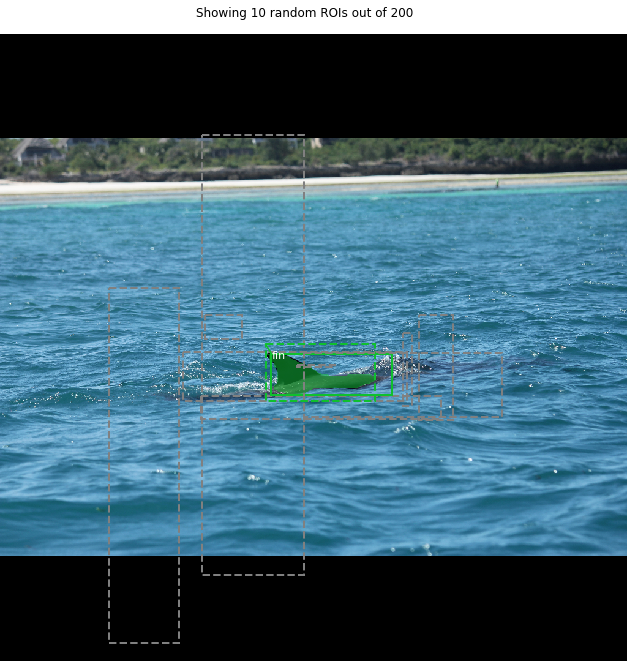
\includegraphics[scale=0.45]{Chapter2/figs/rpn-ten-random.png}
	\end{center}
	\caption{An example of RoIs generated on an image by an RPN, showing 10 random proposals out of the 200 generated. Note that two of the RoIs have been successfully classified as \texttt{fin}.}
	\label{fig:rpn-randoms}
\end{figure}

Selection search is most commonly used with the R-CNN object detection algorithm \cite{girshick_rich_2014}. This algorithm has a high recall rate due to the large amount of proposals, as there is a high probability that some of these proposals will contain Regions of Interest (RoIs) containing the objects being searched for. However, this can be time consuming and computationally expensive (although less computationally expensive than just sliding a window over the full image) as the network needs to be trained to classify these 2000 region proposals, taking up a large amount of disk space. Detection can also be slow using a vanilla R-CNN and, with the selection search being fixed, no adaptive learning takes place here which may lead to bad region proposals throughout. 

Some of these time drawbacks were fixed in later versions of R-CNN, known as Fast-RCNN \cite{girshick_fast_2015}. Rather than feeding the region proposals generated to the CNN, this algorithm instead feeds the input image to the CNN and generates a convolutional feature map. RoIs can then be taken from the feature map using selection search and warped into a shape suitable for the pooling layer, before being reshaped again into a fixed size for the fully connected layer. This is advantageous as it allows us to reuse some computations and allows for backpropagation to occur throughout the network, greatly improving run times.  This also means however that the runtime is dominated by how fast RoIs can be generated. 

To fix this issue, Faster R-CNN was developed \cite{ren_faster_2015}. Now, instead of utilising selection search to generate the RoIs we can utilise a separate network to predict RoIs which can then be used to classify images within the regions. With this, we now train with four losses; 

\begin{enumerate*}
	\item An object/not object classification from the RPN,
	\item The RoI shift,
	\item The object classification,
	\item Final bounding box co-ordinates.
\end{enumerate*}

\subsubsection{Detection Without Proposals}\label{ch:Background,sec:objectDetection,sub:noProposals}

One issue with all RPNs is that they generally take a significant amount of time in order to classify objects in images, with the bottleneck being the region proposal generation. Because of this, there are algorithms which attempt to remove the region proposals altogether and instead look at the whole image. This input image is divided into an equal size grid. Within each square of the grid, we take a set number of bounding boxes which the CNN provides classification confidences for. Any above a set threshold are used to locate the object within the image. These algorithms are essentially one large CNN rather than splitting into a CNN and an RPN and are thus much faster although are not as accurate, especially on smaller objects due to the spatial constraints of the algorithm. Examples of detection without proposal systems include YOLO \cite{redmon_you_2016} and SSD \cite{liu_ssd:_2016}. 


\subsection{Semantic Segmentation}\label{ch:Background,sec:semanticSegmentation}
Along with object detection, semantic segmentation is one of the key research areas in computer vision. Rather than providing bounding boxes around objects of interest as output, semantic segmenters aim to provide fine-grain categorisation for every pixel in an image, grouping pixels together in object classes known as masks. An example of an image and it's masks can be seen in Figure \ref{fig:masks-example}.

\begin{figure}
	\begin{center}
		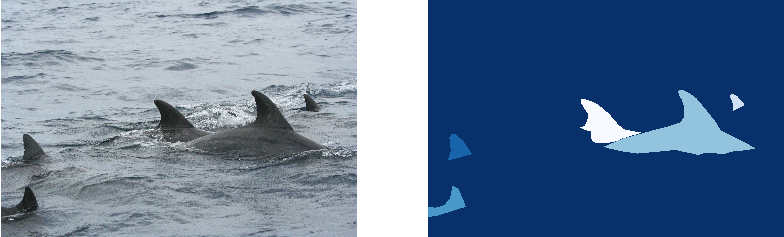
\includegraphics[scale=0.5]{Chapter2/figs/masks-example.png}
	\end{center}
	\caption{An example of an image and it's corresponding ground truth \texttt{fin} masks.}
	\label{fig:masks-example}
\end{figure}

In general, semantic segmenters can be thought of as having two main components; an encoder, usually a pretrained classifier built with a standard detection architecture such as ResNet, and a decoder whose job is to project the coarse grain features learnt by the encoder to a fine-grain pixel space. There are two main ways to approach this decoding step.

The first is to use an RPN to perform region based semantic segmentation, extracting the regions from an image and then describing them. Each pixel of the image is then given a classification based on which highest scoring region it is contained in. Note that any pixels not in a region are given the class label of \texttt{background}. This is achieved through the use of a lightweight binary classifier ran over multiple proposal boxes, known as anchors, covering the image at different scales. Each anchor is given an object score denoted by Intersection Over Union (IOU), a measure of how much overlap there is between a model's predicted bounding box and the ground truth. This is taken at a set confidence threshold, usually 50\%, as the model will predict potentially hundreds of boxes for an image, all with different confidence levels. The vast majority of these predictions will be wrong, but will also (hopefully) have very low confidence scores and so they can be safely ignored and thus not counted in evaluation metrics. Taking a predicted bounding box $B_p$ and a ground truth box $B_g$, the IOU between the two can be defined as:

\begin{equation}
IOU = \frac{\text{Area of overlap}(B_p, B_g)}{\text{Area of union}(B_p, B_g)}
\end{equation}

Anchors with an $IOU >= 0.7$ with any ground truth are donated as positive anchors and are passed on for classification. Those with an $IOU > 0.3$ are considered negative anchors, and those where $0.3 <= IOU < 0.7$ are denoted as neutral anchors and are not used for training. 

\begin{figure}
	\begin{center}
		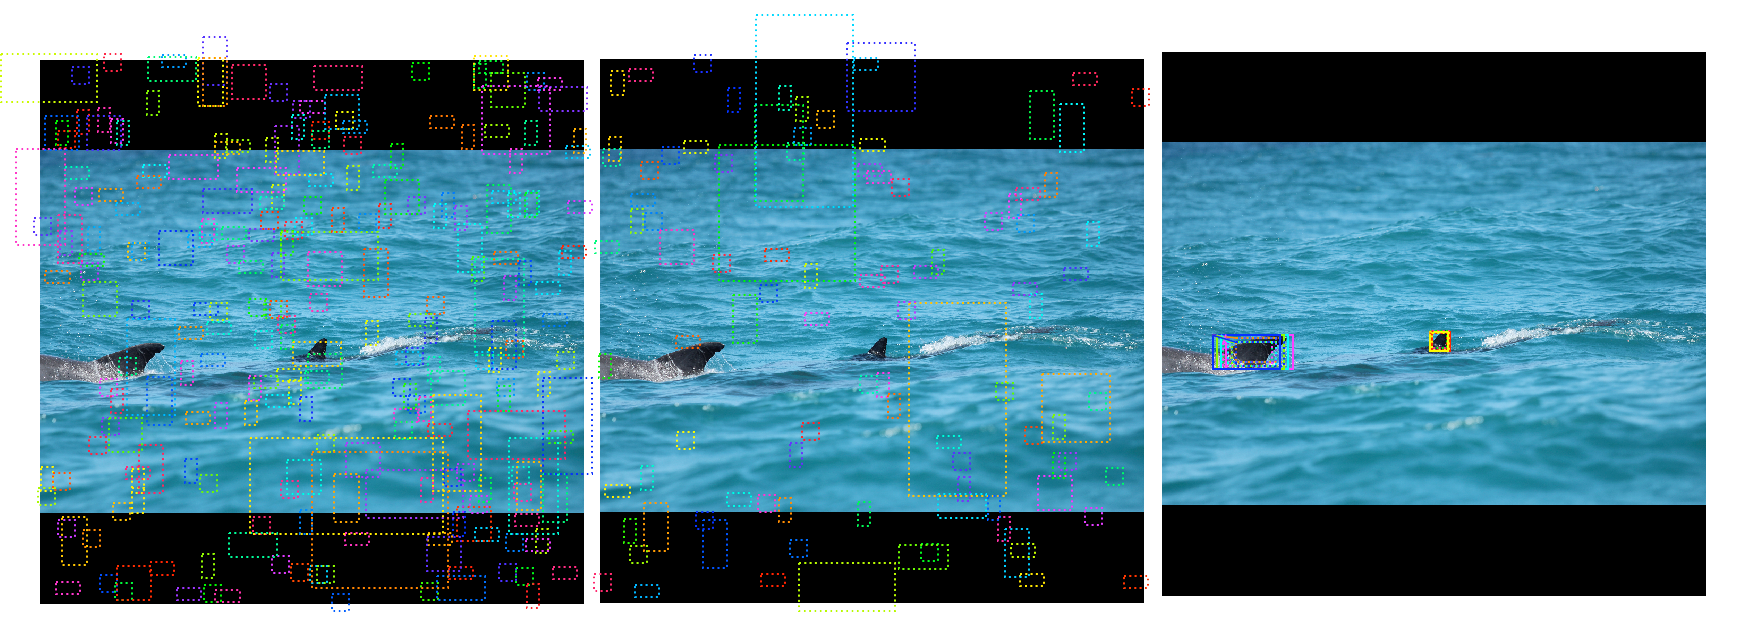
\includegraphics[scale=0.25]{Chapter2/figs/anchor-types.png}
	\end{center}
	\caption{Generated anchors. Left: negative anchors. Middle: neutral anchors. Right: positive anchors.}
	\label{fig:anchor-types}
\end{figure}

Usually however, positive anchors do not fully cover the ground truth object. Because of this, the RPN regresses a refinement applied to the anchors, shifting and resizing them to correct their encasement of the ground truth object. An example of this can be seen in Figure \ref{fig:rpn-refined}.

\begin{figure}
	\begin{center}
		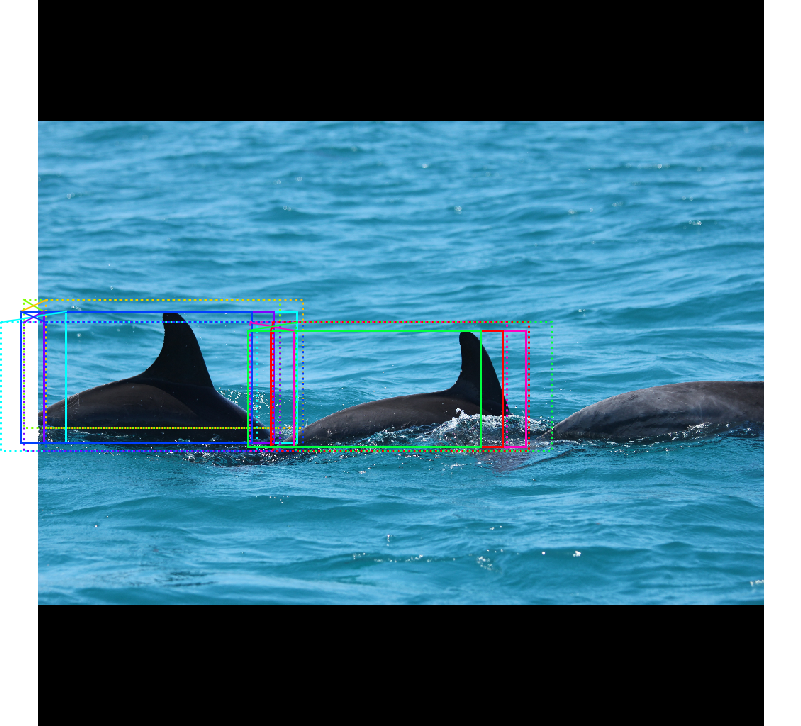
\includegraphics[scale=0.3]{Chapter2/figs/rpn-refined.png}
	\end{center}
	\caption{An example of refined anchors. Positive anchors before refinement are dotted, after refinement are solid.}
	\label{fig:rpn-refined}
\end{figure}

Utilising RPNs does have disadvantages however. Generating the segmentations from the regions take a significant amount of time, and the features generated by RPNs generally do not contain enough feature information to generate well defined masks. Recent research has attempted to fix these issues, such as SDS \cite{hariharan_simultaneous_2014} or Facebook's Mask R-CNN \cite{he_mask_2017}.

Second, a Fully Convolutional Network (FCN) can be utilised for semantic segmentation \cite{long_fully_2014}. An FCN learns pixel to pixel mappings without the need for region proposals, whilst also only including convolutional and pooling layers, allowing for an input image of arbitrary size (compared to classical CNNs which are generally constrained by a preset image size). This does lead to the disadvantage of down sampling the resolution of the outputted feature maps, leading to sometimes ill-defined segmented boundaries. This issue has attempted to be corrected however with more advanced FCNs such as SegNets \cite{badrinarayanan_segnet:_2015} and DeepLab \cite{chen_semantic_2014}. 

Semantic segmentation can be aided through forms of supervised learning. Providing training images which have been given pixel by pixel segmentation masks can greatly improve segmentation class accuracy. Creating these masks can be extremely time consuming for researchers, and is often farmed out to external companies such as Amazon's Mechanical Turk \cite{buhrmester_amazons_2011}.

\subsection{Part Segmentation}\label{ch:Background,sec:Fine-grainedCV,sub:PartSegmentation}
Whilst fine-grained visual categorisation is still an area of new research, an emerging approach to tackling this problem is through the use of part segmentation, whereby a coarse-grained classification is broken down into sub-components which are then analysed to provide a fine-grained identification \cite{zhang_part-based_2014}. This is still an active area of research, with some approaches focusing on a form of hierarchical part matching \cite{xie_hierarchical_2013}, some on alignment of objects to define a super-class shape \cite{gavves_fine-grained_2013}, some utilising deformable part descriptors \cite{zhang_deformable_2013}, and others using part localisation \cite{liu_dog_2012}.


\subsection{Instance Segmentation}\label{ch:Background,sec:instanceSegmentation}

Building on the concept of semantic segmentation, instance segmentation can be performed when further detail about an image is required by a developed system. Whilst many of the underlying processes are similar between the two segmentation types, instance segmentation allows for the model to distinguish between multiple objects which are of the same class;  an example of this can be seen in Figure \ref{fig:instance-vs-semantic}. 

\begin{figure}
	\begin{center}
		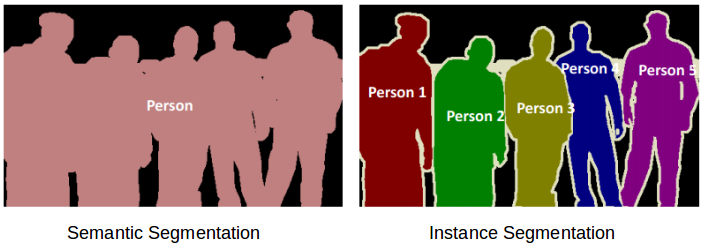
\includegraphics[scale=0.5]{Chapter2/figs/semantic_vs_instance_segmentation.png}
	\end{center}
	\caption{An example showing the difference between semantic and instance segmentation. In semantic segmentation, all pixels which belong to the \texttt{person} class have been classified as one \texttt{person} object. In instance segmentation, five \texttt{person} objects have been detected, and all \texttt{person} pixels have been assigned to one of the objects. Image from \cite{sharma_image_2019}.}
	\label{fig:instance-vs-semantic}
\end{figure}

As such, instance segmentation provides a far more detailed explanation of the input image. This information can be invaluable if your developed system is required not only to understand what pixel classes are present in the input image, but also how many of these class instances there are. In a sense, instance segmentation can be seen as combining both object detection and semantic segmentation into one task. Traditionally however, in order to achieve the goal of instance segmentation, proposed systems have kept the two tasks divided. These \textit{traditionalist} methods take one of two approaches. 

The first, known as \textit{top-down}, begins by detecting objects of interest via an RPN to create bounding boxes. These detections are then fed to the mask predictor to determine which pixels inside of the box belong to either the target or background class. Examples of \textit{top-down} approaches include Faster R-CNN \cite{ren_faster_2015}, and Mask R-CNN \cite{he_mask_2017}. In contrast, \textit{bottom-up} systems first segment then detect, such as SpatialEmbedding \cite{neven_instance_2019} which attempts to tackle instance segmentation through the use of a Gaussian function to produce a probability for a pixel being part of the background or foreground, and then performing object detection on the foreground pixels. \textit{Bottom-up} approaches often fail to reach similar levels of performance as \textit{top-down} approaches however, and are thus rarely used. The major similarity between both \textit{top-down} and \textit{bottom-up} approaches is that they are both sequential in nature, requiring one stage to happen before the other. As such, these systems are very hard to speed up and are far from real-time. However, two stage systems often perform the best in terms of accuracy, and thus are still extremely common backbones of systems requiring the use of instance segmentation. 

In recent years research into the development of real-time instance segmentation has shifted to utilising a one stage approach. These one stage systems are often able to achieve near real-time performance, although often do not produce levels of segmentation accuracy seen when utilising two stage systems. ExtremeNet \cite{zhou_bottom-up_2019} works to extract four "extreme points" and one "center point" of potential objects in the input image through the use of a keypoint estimation network, creating a coarse mask. ESE-Seg \cite{xu_explicit_2019} utilises the concept of Chebyshev polynomials to fit a radius around each object inside of the detected bounding box. Similarly, PolarMask \cite{xie_polarmask_2020} also represents masks through the use of a contour around the object, modelling this through the use of polar coordinates. FourierNet \cite{riaz_fouriernet_2020} builds on this radius concept further through the use of a Fourier transform to smooth the contour. This contouring of the object is extremely fast, however the generated masks are very imprecise. Further, any objects which contain spaces or holes, such as doughnuts, would not be able to be accurately represented. 

YOLOACT \cite{bolya_190402689_2019} builds on the well known YOLO object detection architecture, specifically YOLOv3 \cite{redmon_yolov3_2018}, adding a branch for mask prediction, but performing this through the use of two parallel tasks. The first utilises an FCN to generate prototype masks, whilst the second predicts instance coefficients. These can be combined into one mask through matrix multiplication operations with the detected bounding box. BlendMask \cite{chen_blendmask_2020} works in a similar way to YOLOACT however predicts an attention map rather than instance coefficients and utilises FCOS \cite{tian_fcos_2019} as a backbone, a completely anchor and proposal free object detection architecture resulting in reduced complexity when compared to YOLO \cite{redmon_you_2016} and SSD \cite{liu_ssd:_2016}. 

Whilst the majority of one stage approaches to instance segmentation rely on bounding boxes, this is not always the case. SOLO \cite{wang_solo_2020} introduces the concept of instance categories, assigning categories to each pixel according to the size and location of the instance. SOLOv2 \cite{wang_solov2_2020} builds on SOLO through the implementation of an novel non-maximum suppression algorithm. SOLOv2 often depicts higher quality masks than more often used two-stage systems such as Mask R-CNN and is able to perform real-time inference, although it should be noted that both SOLO and SOLOv2 are extremely recent additions to the instance segmentation arsenal, both being released in 2020. 

\subsubsection{Mask R-CNN}\label{ch:Background,sec:instanceSegmentation,sub:Mask R-CNN}

As discussed in previous Sections, there are multiple standardised architectures utilised for segmentation tasks. As such, when developing a system which utilises segmentation developers of these systems will, more often than not, use one of the many architectures from literature rather than developing their own custom architecture. Utilising one of the standard architectures has many advantages; for one, researchers do not need to spend time creating a model architecture for their task, allowing for development in other, novel areas. Further to this, utilising a standard architecture allows for research to be more easily understood and reproduced. As this thesis focusses on the automation of photo-identification systems rather than on the development of new novel architectures, it makes sense to make use of an architecture which is well known, has a track record of performing well when trained on non-benchmark or custom datasets, and is easily reproducible. As such, parts of this project's automation pipeline make use of Mask R-CNN \cite{he_mask_2017}. Because of this, it is important to understand Mask R-CNN in more detail compared to the other architectures discussed previously in this Chapter. 

As we have seen previously, it is often the case that new architectures either extend or borrow features from older ones. This is also the case with Mask R-CNN. Developed in 2017 by He \textit{et al.} at Facebook AI Research, Mask R-CNN was developed on top of the existing 2016 Faster R-CNN architecture from Ren \textit{et al.} \cite{ren_faster_2015} (itself an extension of Fast R-CNN developed in 2015 \cite{girshick_fast_2015}). 

Faster R-CNN is a two stage architecture. The first stage utilises a standard backbone network, typically ResNet \cite{he_deep_2015}, VGG \cite{simonyan_very_2015}, or Inception \cite{szegedy_going_2015}, to convert an input image into a set of feature maps which are passed to an RPN for analysis (see Section \ref{ch:Background,sec:objectDetection,sub:RPN} for a breakdown of RPNs). This RPN generates region proposals which are passed to the second stage of Faster R-CNN, along with the previously generated feature maps, and fed to an RoI pooling layer.  Here, each proposed region and corresponding feature map is utilised to predict bounding boxes, classifications, and confidence scores. A visual representation of Faster R-CNN's architecture can be seen in Figure \ref{fig:faster-r-cnn-architecture}.


\begin{figure}
	\begin{center}
		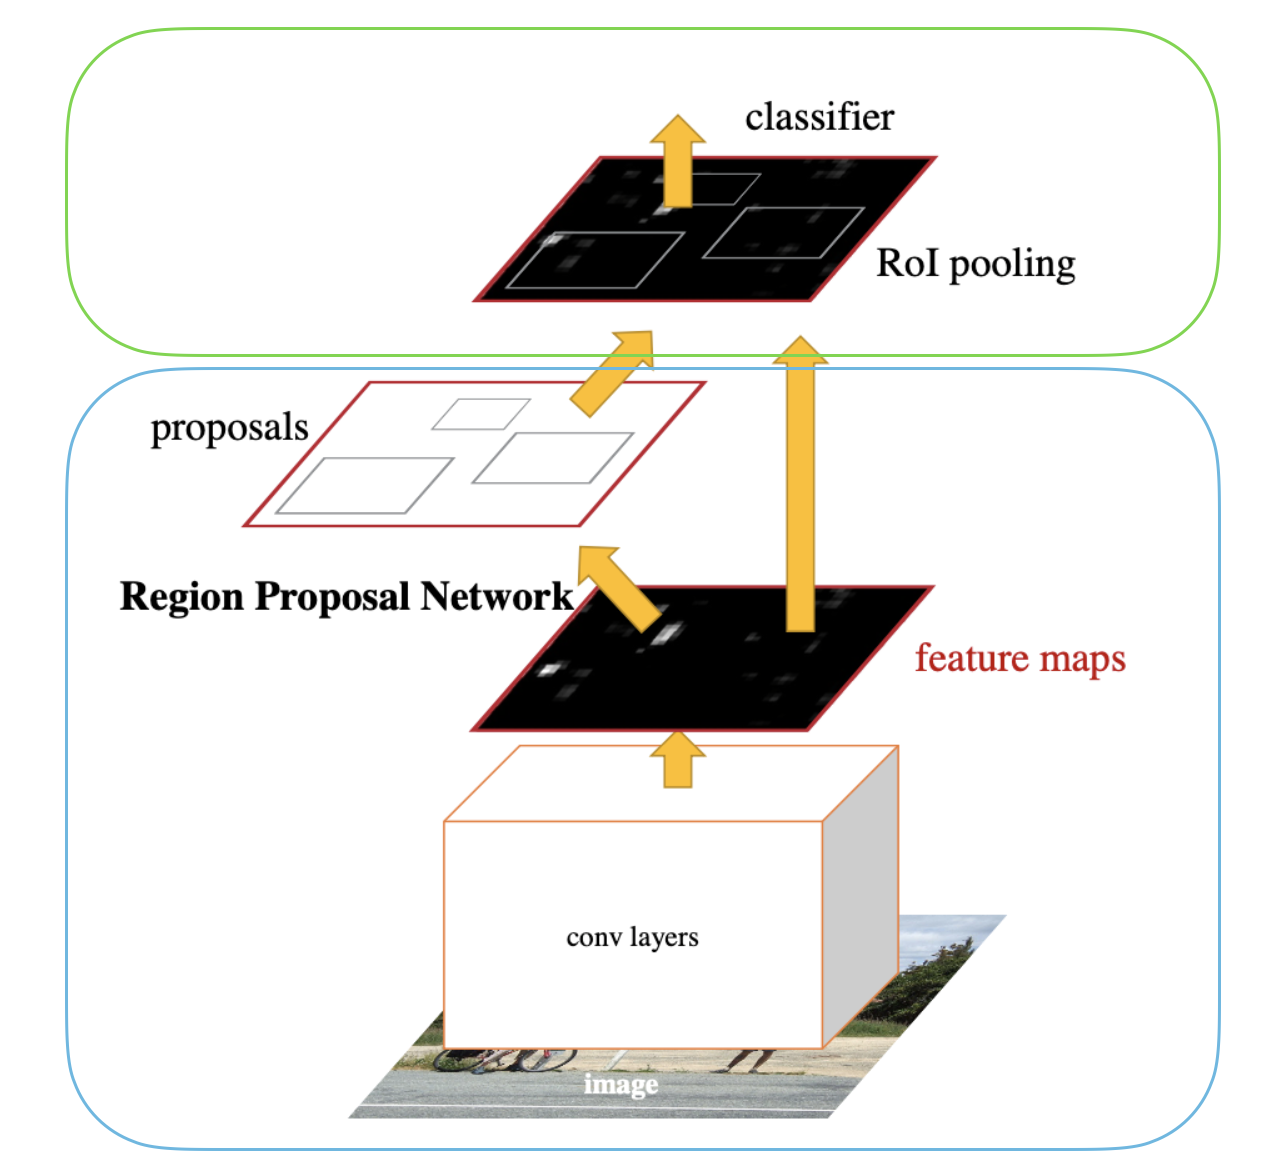
\includegraphics[scale=0.3]{Chapter2/figs/faster-r-cnn-architecture.png}
	\end{center}
	\caption{The Faster R-CNN architecture \cite{ren_faster_2015}. The blue box represents operations in stage one. The green box represents operations in stage two.}
	\label{fig:faster-r-cnn-architecture}
\end{figure}


Mask R-CNN extends Faster R-CNN, allowing for instance segmentation through some relatively simple changes and additions to stage two of the architecture. First, the RoI pooling layer is replaced with an RoI align layer. This replacement layer removes the "harsh quantisation" which is present in RoI pooling, and properly aligns the extracted features with the input image. Second, an additional branch is added to the end of stage two. This branch receives the output of the new RoI align layer and processes it using a \textit{mask head}, consisting of additional convolutional layers which generate pixel predictions and instance mask outputs. See Figure \ref{fig:mask-r-cnn-changes} for a visual representation of the changes made by Mask R-CNN.  

\begin{figure}
	\begin{center}
		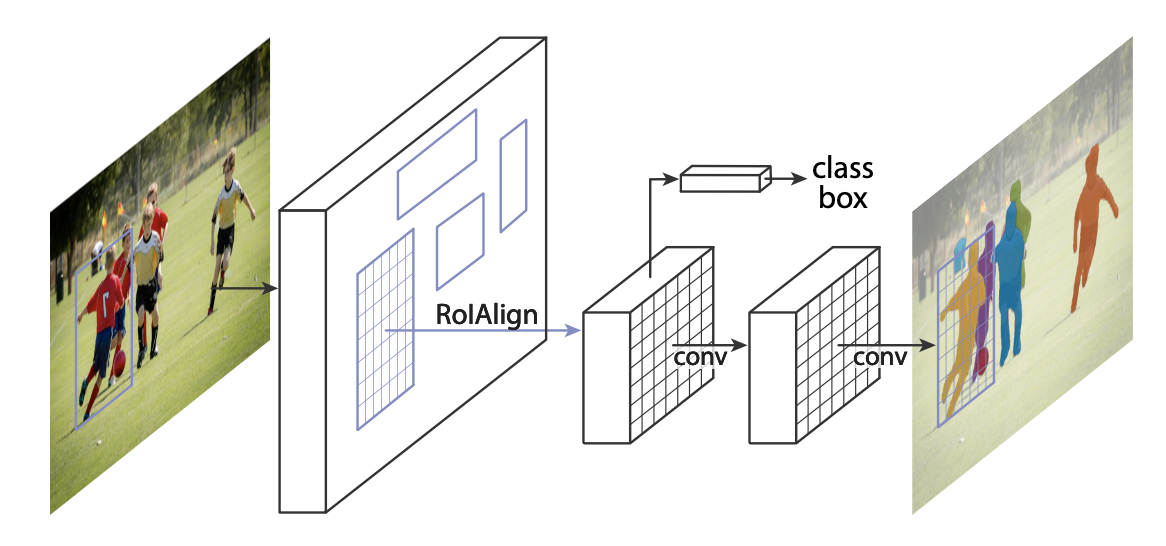
\includegraphics[scale=0.3]{Chapter2/figs/mask-r-cnn-changes.png}
	\end{center}
	\caption{A visual representation of the changes made to Faster R-CNN to create Mask R-CNN. \cite{he_mask_2017}}
	\label{fig:mask-r-cnn-changes}
\end{figure}

Thanks to these additions, Mask R-CNN is able to perform extremely accurate instance segmentation with a relatively small drop in inference speed. Whilst it is not real-time, this is an acceptable trade off for the accuracy of predictions on custom datasets. Indeed the use of Mask R-CNN for instance segmentation in literature is far ranging, being utilised in medical \cite{rohit_malhotra_autonomous_2018, chiao_detection_2019, liu_segmentation_2018, anantharaman_utilizing_2018}, agriculture \cite{qiao_cattle_2019, zhao_comparing_2018, lee_potato_2020, chu_deepapple_2020}, sports \cite{buric_ball_2018, pobar_detection_2019, nguyen_hand_2018}, astronomy \cite{burke_deblending_2019}, and nautical \cite{nie_inshore_2018, hong_trashcan_2020} fields. As well as being well known, Mask R-CNN is also extremely reproducible. An official PyTorch implementation is available through Facebook AI Research's Github \cite{wu_detectron2_2020}, whilst Matterport's Mask R-CNN implementation is most commonly utilised when working with Tensorflow (including in this project) \cite{waleed_mask_2017}.

\subsection{Fine-Grained Visual Categorisation}\label{ch:Background,sec:Fine-grainedCV}

Categorisation of objects through the use of machine learning may at first glance look like a solved problem. Indeed, it is now possible to achieve extremely high levels of accuracy on a wide variety of tasks; at the time of writing the current state of the art for ImageNet \cite{institute_of_electrical_and_electronics_engineers_2009_2009} and CIFAR-10 \cite{krizhevsky_learning_2009}, two of the most commonly used classification benchmark datasets, are both held by Foret \textit{et al.} utilising EfficinetNet with SAM \cite{foret_sharpness-aware_2020} at 88.61\% and 99.70\% top-1 accuracy respectively. Even outside of these benchmarks however, high accuracies would be expected for more complex use cases where custom datasets have been created, such as in manufacturing environments. However, it is important to note that all of these tasks are coarse-grain in nature. Benchmark datasets usually contain classes which are relatively distinct, for example \texttt{cat}, \texttt{dog}, and \texttt{ship} classes in CIFAR-10, which all have large interclass variation. 

In more recent years the focus of research in object detection has thus mostly shifted from the coarse-grain to the fine-grain domain, where distinct classes have small interclass variation. For example whilst CIFAR-10 has one class covering all different types of \texttt{dog}, the fine-grain dataset Stanford Dogs \cite{khosla_novel_2011} is made up of 120 classes each containing examples of only one dog breed each (\texttt{chihuahua}, \texttt{beagle}, etc.). Other common fine-grain benchmark datasets often focus on wildlife or vehicles, including Caltech-UCSD Birds 200 \cite{welinder_caltech-ucsd_2010} and the updated Caltech-UCSD Birds 200-2011 \cite{wah_caltech-ucsd_2011}, iWildcam for camera trap data \cite{beery_iwildcam_2019}, and FGVC Aircraft \cite{maji_fine-grained_2013}. 

Whilst fine-grain datasets may contain small inter-class variation, their intra-class variation is often large. Class examples often contain a wide variety of orientations, poses, colour, and sizes. This allows for trained models to be more generalisable and capable of detecting class examples in previously unseen images where the example may be obscured or unlike conventional class examples. It is also important to note here that models which perform well on coarse-grain data are not guaranteed to do so on fine-grain data. For example EfficientNet with SAM which, as previously stated, is state of the art in multiple coarse-grain tasks currently ranks 31\textsuperscript{st} in the FGVC Aircraft benchmark ranking on Papers With Code \footnote{Papers With Code - FGVC Aircraft Rankings: \href{https://paperswithcode.com/sota/fine-grained-image-classification-on-fgvc}{paperswithcode.com/sota/fine-grained-image-classification-on-fgvc}}.

\section{Computer Vision for Conservation Technology}\label{ch:Background,sec:conTech}

Thanks to the large advancements in computer vision and deep learning, and the increasing prevalence of these systems in areas such as manufacturing and healthcare, researchers have, in recent years, began exploring other areas of society which could benefit from AI systems. One of the more niche, but arguably highly important areas where computer vision can make an impact, is conservation \cite{weinstein_computer_2018}.

Work in conservation tech has been mostly dominated by machine learning systems for camera traps. This makes sense, as this data collection technique usually operates over vast spatial and temporal areas. As such, a large amount of varied data already exists for systems to be trained on. For example, the Snapshot Serengeti project \footnote{Snapshot Serengeti: \href{https://www.snapshotserengeti.org/}{snapshotserengeti.org}}, developed by Swanson \textit{et al.} has utilised camera traps in Tanzania's Serengeti National Park to develop a fully labelled camera trap image dataset capable of training machine learning systems. The camera traps used have been in continuous operation since 2010 and cover an area of 1125km\textsuperscript{2} \cite{swanson_snapshot_2015}. The iWildcam dataset provides further camera trap training data from across the South-western United States \cite{beery_iwildcam_2019}.

 A second advantage of camera trap data is their high false positive rate. These traps capture a photo every time movement in the frame is detected, and as such a large proportion of the images a camera trap captures either do not contain any animals at all (e.g. wind has caused the surrounding vegetation to move), or contain animals which are not the primary species of investigation. This large false positive rate provides a key driver for the development of machine learning camera trap systems which could, for example, filter out these false positive captures automatically. Whilst these images may simply be discarded by the researchers, they have a use in the development of machine learning camera trap based systems, allowing the system to be trained on a wide variety of false positive examples. As such, machine learning systems developed for camera traps have found quick adoption in the conservation community with many systems now capable of performing fine-grained species classification with extremely high accuracy \cite{tabak_machine_2019, norouzzadeh_automatically_2018, willi_identifying_2019, beery_efficient_2019, norouzzadeh_deep_2019}. Recent work by Clapham \textit{et al.} has moved further to the extreme of fine-grained classification with BearID, a project which adapts human facial recognition systems for use with brown bears (\textit{Ursus arctos}) via metric embeddings, achieving an ``individual classification accuracy'' of 83.9\%. Here, BearID is not classifying the species \textit{Ursus arctos} but rather individuals within the \textit{Ursus arctos} population, a significant achievement given the challenge of identifying individuals within a species which do not have unique markings \cite{rowcliffe_estimating_2008}.

Marine conservation researchers, in contrast to their on-land counterparts, have been slower at adopting computer vision to aid their research. This is, in part, due to the relative lack of available data to train systems. Due to the unsuitability of marine environments for the deployment of camera traps, conservationists here traditionally rely on identification from photographs taken either from the coastline or from a vessel. As this requires a human operator, the size of datasets available is relatively small. Furthermore, given the high cost of data collection, marine conservation groups often keep a tight grip on their data. This has led to a lack of available open-source datasets for those who wish to train machine learning systems for use in marine conservation. Thanks to advances in UAV technology and their current inexpensiveness, some research groups have shifted focus to the use of drones for image capture. This new approach has seen success in areas such as photo-identification \cite{bogucki_applying_2019, gray_drones_2019}, microbial sampling \cite{centelleghe_use_2020}, and human-interaction response monitoring \cite{fiori_using_2020}. The use of drones for this time of work is not yet mainstream however, and some recently published work highlights the need to better understand how drones affect the behaviour and health of marine species \cite{giles_responses_2020, bevan_measuring_2018, ramos_bottlenose_2018, pomeroy_assessing_2015}. 

\subsection{Utilising Computer Vision in Cetacean Conservation}\label{ch:Background,sec:conTech,sub:cetaceanDetection}

The idea of utilising statistical methodology and machine learning in a marine cetacean space has, in recent years, been gaining popularity, with multiple papers being published in this area. Karnowski \textit{et al.} propose using Robust PCA to subtract background from underwater images to help identify captive bottlenose dolphins, and track their movements through multiple distinct areas, allowing researchers to annotate pool positions 14 times faster than before \cite{karnowski_dolphin_2015}. Bouma \textit{et al.} provide a system focusing on metric embedding learning to photo-id individual common dolphins, achieving top-5 accuracy scores of around 93\% \cite{bouma_individual_2018}. Further, Qui\~{n}onez \textit{et al.} propose a CNN based system to detect four classes: \texttt{dolphin}, \texttt{dolphin\_pod}, \texttt{open\_sea}, and \texttt{seabirds} \cite{quinonez_using_2019}. 

Outside of statistical theory and academic papers, multiple systems have been developed, or are currently in development, to aid cetacean researchers in the photo-id process. The first of these, known as FinScan, was developed in 2000 \cite{hillman_finscan_2002}. This is a semi-automated photo-id assistant whereby the user imports images taken during fieldwork which FinScan then attempts to create a trace of the fin in the image. Users may manually edit this trace however if it is not exact (this feature was developed due to frustration with barnacles attaching to fins in the area where FinScan was developed). This trace of the fin is then checked against a local Microsoft Access database to determine close matches which are presented to the user. Before images are imported into FinScan they must be manually cropped, sharpened, and rotated by the user. Rotation of the image is especially important, and the FinScan algorithm is not rotation invariant. Further to this due to FinScan being an old piece of software, whilst it is freeware it is no longer readily available. Anyone who wishes to use it must procure a copy from someone else, there is no central repository for downloading. Issues with running the software on newer systems may also be present.

Similarly to FinScan, FinBase is a photo-id database management system developed by NOAA Fisheries \cite{fisheries_finbase_2018}. However, unlike other systems, FinBase provides no matching based on automatically generated fin properties; instead, FinBase facilitates matching through user defined attributes. These could be physical descriptors such as `top notch' or `skin disorder' but may also be non-physical attributes if the user wishes. Fins are partially matched based on querying the backend database for entries which also have the attributes of those inputted by the user for the query fin. 

Alongside both of these, DARWIN \cite{hale_unsupervised_2012} provides automated identification of new images based on those already in the attached database. Like FinScan, users of DARWIN trace around the leading and trailing edges of the fin they wish to identify. These edges are stored in a database as a set of evenly spaced points approximating the outline of the fin which is then used for identification.

Photo-ID Ninja\footnote{Photo-ID Ninja: \href{http://photoid.ninja}{photoid.ninja}} is a system currently in development which aims to photo-id individuals based on pigmentation commonly found on fins of the New Zealand common dolphin (\textit{Delphinus} spp.) \cite{gilman_computer-assisted_2016}. Here, pigmentation is used due to the low chance of other prominent markings becoming present on individuals. Matching is performed via the Euclidean distance between the input image and the catalogue of known individuals, which is then sorted by ID and validated using 5 fold cross-validation \cite{bouma_individual_2018-1}. Current reported accuracies for this pigmentation matching are a top-1 accuracy of 90.6\%, top-5 accuracy of 93.6\%, and an mAP of 80.8\%. This pigmentation matching is still in development however, although Photo-ID Ninja does currently provide a bulk cropping mechanism to aid in the speed up of manual identification. Users can provide a batch of images taken directly from the field to the system, which then outputs a zip file of cropped fins which can then be manually identified. 

Work undertaken by Georgetown University and Google in the area of cetacean photo-id has also provided promising results \cite{mann_mann-urian-google_2019, georgetown_university_is_2018, liang_googles_2018}. The system, which utilises Google's Cloud Auto ML framework, can quickly identify bottlenose dolphins from Australia's Shark Bay. This system shows users the top-200 closest matches along with their confidence scores utilising both the leading and trailing edges of the fin. It is reported that this system saves Georgetown University's cetacean team around 4500 hours per year, highlighting the need for systems such as these to researchers in this field. However, this system does not link to a backend database to log matches found - this must be done manually by the researchers. Further, any new individuals which need to be added to the system, or indeed if the system was to be redeployed to a new area, then all training of the underlying model must be performed by Google engineers rather than locally by the researchers who wish to utilise the system. Further, fins to be identified must be inputted one by one, no batch input function exists.  

In the past few years, systems utilising CNNs have started to enter the photo-id space. HappyWhale\footnote{HappyWhale: \href{https://happywhale.com/}{happywhale.com}} is a CNN based photo-id system focussing on humpback whales (\textit{Megaptera novaeangliae}). The underlying CNN for this system was developed through a Kaggle competition\footnote{Kaggle competition: \href{https://www.kaggle.com/c/whale-categorization-playground}{kaggle.com}} by user Jinmo Park to identify patterns present on the tailstock of the humpbacks \cite{kaggle_humpback_2018}, utilising elements of ArcFace \cite{deng_arcface_2019} and DeepFace \cite{taigman_deepface_2014} to do so. Users interact with HappyWhale through their website, uploading images of the tailstocks encountered. The HappyWhale system then attempts to identify the individual before presenting back to the user. If the user provides location data, HappyWhale also keeps track of this to produce travel maps for the individuals, as humpback whales are known to travel vast distances in their lives. Success rate for HappyWhale varies greatly, from 99\% for "good to high quality" images to 50\% for full fins at 50x50px. HappyWhale struggles with partially obscured tailstocks however, and work is currently ongoing in this area \cite{cheeseman_ted_2019}. 

Of all the systems in use or development today, one of the largest and most well known is FlukeBook\footnote{FlukeBook: \href{https://www.flukebook.org/}{flukebook.org}}, a fully automatic photo-id system for bottlenose dolphins, humpback whales, and sperm whales (\textit{Physeter macrocephalus}). This system is part of a wider network of animal identification tools based on Wildbook, an open source software framework developed by non-profit organisation WildMe to facilitate the introduction of artificial intelligence into the conservation space \cite{berger-wolf_wildbook:_2017}. Within FlukeBook there are two main photo-id algorithms; CurvRank and FinFindR.

CurvRank is an algorithm developed by Weideman \textit{et al.} \cite{weideman_integral_2017} which automatically identifies the trailing edge of the fin and represents this as a set of ordered coordinates. Each coordinate point then has a circle of radius $r$ placed upon it, before being transformed horizontally. The curvature at this point for a given $r$ value is then defined as the ratio of the area under the curve againsy the area of a square around the curve of length $2r$. This allows for the definition of the trailing edge of the fin to be rotation invariant. 

FinFindR is an algorithm developed by Thompson \textit{et al.} which allows for inputted images containing bottlenose dolphins to be identified. FinFindR works with uncropped images of the whole area unlike other systems which require just the fin to be in the image. FinFindR then automatically detects the dolphin and crops it out, saving a new image. Cropping can be performed on either the whole body or on the dorsal fin only. This cropped image is then passed to a canny edge detector which creates an embedding of the trailing edge of the fin. This embedding is mapped into a high dimensional space based on work in FaceNet \cite{schroff_facenet_2015}, with clustering of individuals achieved using Ward's variance minimising clustering \cite{ward_hierarchical_1963}. Reported accuracies for FinFindR currently stand at a top-1 accuracy of 88\%, top-5 accuracy of 94\%, and top-50 accuracy of 97\% \cite{thompson_finfindrpdf_2019}. It should be noted however that FinFindR has currently only been tested on bottlenose dolphins and work is still ongoing. The code for FinFindR can be found on GitHub \footnote{FinFindR: \href{https://github.com/haimeh/finFindR}{github.com/haimeh/finFindR}}.

Recent work undertaken by Lee \textit{et al.} proposes a novel algorithm for cetacean identification \cite{lee_backbone_2020}. The proposed system is capable of detecting small objects in large images, and utilises this for fin detection. Next, segmentation is performed using U-Net \cite{ronneberger_u-net_2015}. The resultant output is then passed to a post processor which re-aligning and normalising the fin. The most significant features of the fin are then extracted and passed to a VGG based system \cite{simonyan_very_2015}, combined with a novel V2BC component, for identification. 

Maglietta \textit{et al.} propose DolFin \cite{maglietta_dolfin_2018}, a SURF based system \cite{bay_speeded-up_2008} building upon work undertaken by Renò \textit{et al.} \cite{reno_sift-based_2019} for identifying Risso's dolphins. As mentioned in Section \ref{ch:Background,sec:photo-id}, this species is susceptible to prominent long-term scarring, and thus is well suited to feature detection algorithms such as SURF, with published results showing a much greater identification accuracy can be achieved compared to utilising common photo-id aides such as DARWIN \cite{hale_unsupervised_2012}.  


%%%%%%%%%%%%%%%%%%%
\nomenclature[z-CNN]{CNN}{Convolutional Neural Networks}
\nomenclature[z-CV]{CV}{Computer Vision}
\nomenclature[z-CPU]{CPU}{Central Processing Unit}
\nomenclature[z-GPU]{GPU}{Graphical Processing Unit}
\nomenclature[z-SGD]{SGD}{Stochastic Gradient Descent}
\nomenclature[z-ReLU]{ReLU}{Rectified Linear Unit}
\nomenclature[z-FCN]{FCN}{Fully Convolutional Network}
\nomenclature[z-RPN]{RPN}{Region Proposal Network}
